\documentclass
[kulak] % [kulak|kul|kuleuven-brugge,handout|outline|]
{kulakbeamer}

\usepackage[dutch]{babel}
\usepackage[T1]{fontenc}
\usepackage{tikz}
\usepackage{pgfplots}	
\pgfplotsset{compat=newest}   % or a specific version, e.g. 1.18
\usepackage{pgfmath}
\usepackage{graphicx}
\usepackage[dutch]{babel}
\usepackage{subfiles}
\usepackage{amssymb, amsthm, amsmath,hyperref,mhchem,siunitx}
\sisetup{output-decimal-marker = {,}}
\usepackage[section]{placeins}
\usepackage[gen]{eurosym}
\usepackage{multicol}

\title[Bachelorproef]{Bachelorproefvoorstelling van grafenkleuringen}
\subtitle{Ondertitel}
\author{Arne Claerhout} 
\institute[Kulak]{KU Leuven Kulak}
\date{Academiejaar 2025 -- 2026}

\renewcommand{\outlineTitle}{Overzicht} % enkel met optie outline

\begin{document}
	
	\begin{titleframe}
		\titlepage
	\end{titleframe}
	
	\begin{outlineframe}[Overzicht]
		\tableofcontents
	\end{outlineframe}
	
	
	\section{Inleiding}
	
	\begin{frame}
		\frametitle{Grafenkleuringen}
		
		\begin{multicols}{2}

			\begin{itemize}
				\item Knopen
				\item 4 soorten
				\pause
				\begin{itemize}
					\item Proper kleuring
				\end{itemize}
			\end{itemize}
			
			\vspace*{\fill}\null
			
			\pause
			% This file was created with tikzplotlib v0.10.1.
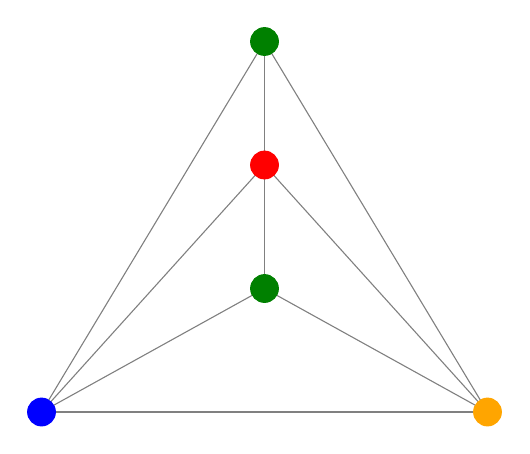
\begin{tikzpicture}

\definecolor{darkgray176}{RGB}{176,176,176}
\definecolor{gray}{RGB}{128,128,128}

\begin{axis}[
hide x axis,
hide y axis,
mark size=5pt,
scaled x ticks=manual:{}{\pgfmathparse{#1}},
scaled y ticks=manual:{}{\pgfmathparse{#1}},
tick align=outside,
x grid style={darkgray176},
xmajorticks=false,
xmin=-1.21, xmax=1.21,
xtick style={color=black},
xticklabels={},
y grid style={darkgray176},
ymajorticks=false,
ymin=-0.505, ymax=0.705,
ytick style={color=black},
yticklabels={}
]
\path [draw=gray]
(axis cs:-1,-0.4)
--(axis cs:1,-0.4);

\path [draw=gray]
(axis cs:-1,-0.4)
--(axis cs:0,-0.0666666666666667);

\path [draw=gray]
(axis cs:-1,-0.4)
--(axis cs:0,0.266666666666667);

\path [draw=gray]
(axis cs:-1,-0.4)
--(axis cs:0,0.6);

\path [draw=gray]
(axis cs:1,-0.4)
--(axis cs:0,-0.0666666666666667);

\path [draw=gray]
(axis cs:1,-0.4)
--(axis cs:0,0.266666666666667);

\path [draw=gray]
(axis cs:1,-0.4)
--(axis cs:0,0.6);

\path [draw=gray]
(axis cs:0,-0.0666666666666667)
--(axis cs:0,0.266666666666667);

\path [draw=gray]
(axis cs:0,0.266666666666667)
--(axis cs:0,0.6);

\addplot [
  mark=*,
  only marks,
  scatter,
  scatter/@post marker code/.code={%
  \endscope
},
  scatter/@pre marker code/.code={%
  \expanded{%
  \noexpand\definecolor{thispointdrawcolor}{RGB}{\drawcolor}%
  \noexpand\definecolor{thispointfillcolor}{RGB}{\fillcolor}%
  }%
  \scope[draw=thispointdrawcolor, fill=thispointfillcolor]%
},
  visualization depends on={value \thisrow{draw} \as \drawcolor},
  visualization depends on={value \thisrow{fill} \as \fillcolor}
]
table{%
x  y  draw  fill
-1 -0.4 0,0,255 0,0,255
1 -0.4 255,165,0 255,165,0
0 -0.0666666666666667 0,128,0 0,128,0
0 0.266666666666667 255,0,0 255,0,0
0 0.6 0,128,0 0,128,0
};
\draw (axis cs:-1,-0.4) node[
  scale=0.6,
  text=white,
  rotate=0.0
]{1};
\draw (axis cs:1,-0.4) node[
  scale=0.6,
  text=white,
  rotate=0.0
]{2};
\draw (axis cs:0,-0.0666666666666667) node[
  scale=0.6,
  text=white,
  rotate=0.0
]{3};
\draw (axis cs:0,0.266666666666667) node[
  scale=0.6,
  text=white,
  rotate=0.0
]{4};
\draw (axis cs:0,0.6) node[
  scale=0.6,
  text=white,
  rotate=0.0
]{3};
\end{axis}

\end{tikzpicture}

			
		\end{multicols}
		
	\end{frame}
	
	\begin{frame}
		\frametitle{Andere kleuringen}
		
		
		\begin{multicols}{2}
			
			\begin{itemize}
				\item Odd coloring
				\begin{itemize}
					\item Proper
					\item Oneven kleur
				\end{itemize}
			\end{itemize}
			
			\vspace*{\fill}\null
			
			\pause
			\begin{center}
				\scalebox{.75}{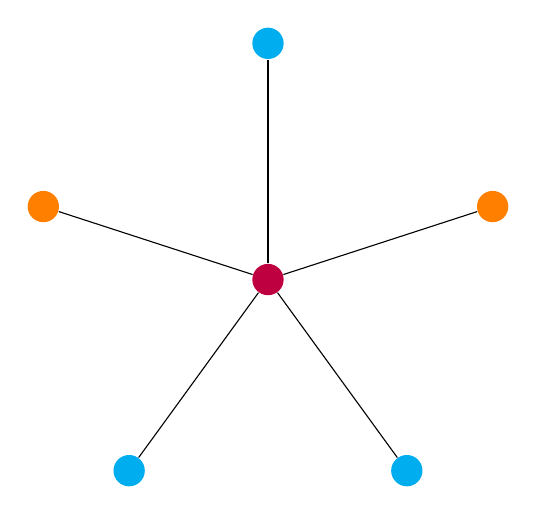
\begin{tikzpicture}[scale=2]
	
	% ---- Adjustable colors ----
	\def\centerColor{purple}
	\def\colorA{cyan}
	\def\colorB{orange}
	\def\colorC{cyan}
	\def\colorD{cyan}
	\def\colorE{orange}
	
	% ---- Positions of outer vertices (5 around a circle) ----
	\foreach \i/\name/\col in {
		90/A/\colorA,
		18/B/\colorB,
		-54/C/\colorC,
		-126/D/\colorD,
		162/E/\colorE
	}
	{
		\node[fill=\col, circle, inner sep=4pt] (v\name) at (\i:1.5) {};
	}
	
	% ---- Center vertex ----
	\node[fill=\centerColor, circle, inner sep=4pt] (center) at (0,0) {};
	
	% ---- Edges to center ----
	\foreach \name in {A,B,C,D,E}
	\draw (center) -- (v\name);
	
\end{tikzpicture}
}
			\end{center}
			
			
		\end{multicols}
		
		
	\end{frame}
	
	\begin{frame}
		\frametitle{Andere kleuringen}
		
		
		\begin{multicols}{2}
			
			\begin{itemize}
				\item Odd coloring
				\begin{itemize}
					\item Proper
					\item Oneven kleur
				\end{itemize}
			\end{itemize}
			
			\vspace*{\fill}\null
			
			\begin{center}
				\scalebox{.75}{\input{exampleOddMiss.tex}}
			\end{center}
			
			
		\end{multicols}
		
		
	\end{frame}
	
	\begin{frame}
		\frametitle{Andere kleuringen}
		
		
		\begin{multicols}{2}
			
			\begin{itemize}
				\item Odd coloring
				\item Conflict free coloring
				\pause
				\begin{itemize}
					\item 4 opsplitsingen
					\item Proper $\longleftrightarrow$ Improper
					\item Open $\longleftrightarrow$ Closed
				\end{itemize}
			\end{itemize}
			
			\vspace*{\fill}\null

			
			\pause
			\begin{center}
%				\scalebox{.75}{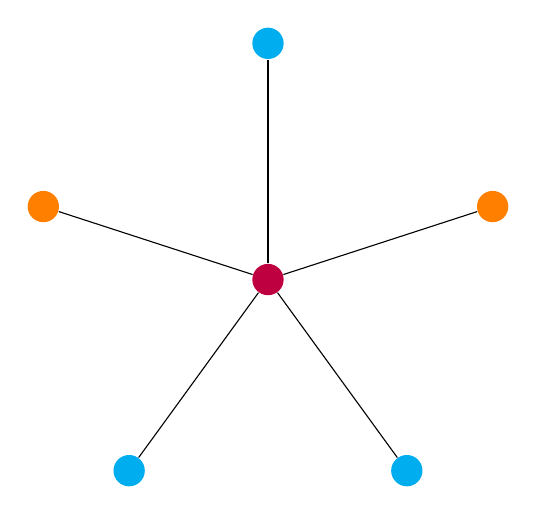
\begin{tikzpicture}[scale=2]
	
	% ---- Adjustable colors ----
	\def\centerColor{purple}
	\def\colorA{cyan}
	\def\colorB{orange}
	\def\colorC{cyan}
	\def\colorD{cyan}
	\def\colorE{orange}
	
	% ---- Positions of outer vertices (5 around a circle) ----
	\foreach \i/\name/\col in {
		90/A/\colorA,
		18/B/\colorB,
		-54/C/\colorC,
		-126/D/\colorD,
		162/E/\colorE
	}
	{
		\node[fill=\col, circle, inner sep=4pt] (v\name) at (\i:1.5) {};
	}
	
	% ---- Center vertex ----
	\node[fill=\centerColor, circle, inner sep=4pt] (center) at (0,0) {};
	
	% ---- Edges to center ----
	\foreach \name in {A,B,C,D,E}
	\draw (center) -- (v\name);
	
\end{tikzpicture}
}
			\end{center}
			
			\vspace*{\fill}\null
			
			
		\end{multicols}
		
		
	\end{frame}
	
	\begin{frame}
		\frametitle{Andere kleuringen}
		
		
		\begin{multicols}{2}
			
			\begin{itemize}
				\item Odd coloring
				\item Conflict free coloring
				\item Unique-Maximum coloring
				\pause
				\begin{itemize}
					\item 4 opsplitsingen
					\item Proper $\longleftrightarrow$ Improper
					\item Open $\longleftrightarrow$ Closed
				\end{itemize}
			\end{itemize}
			

			
			\begin{center}
%				\scalebox{.75}{\input{exampleOddMiss.tex}}
			\end{center}
			
			\vspace*{\fill}\null
			
		\end{multicols}
		
		
	\end{frame}
	
	\begin{frame}
		\frametitle{Literatuur}
		
		\begin{itemize}
			\item Proper conflict-free and unique-maximum colorings of planar graphs with respect to neighborhoods
			\begin{itemize}
				\item Brengt resultaten samen
				\item Voert unique-maximum kleuringen in
			\end{itemize}
			\item Colorings with neighborhood parity condition
			\begin{itemize}
				\item Bewijst bovengrens
				\item Ondergrens door $C_5$
			\end{itemize}
		\end{itemize}
		
		
	\end{frame}
	
	\section{Besluit}
	
\end{document}
